\subsection{The lift of homomorphisms of associated graded modules}

THEOREM 1. Let X, Y be two filtered groups whose filtrations \((\mathbf{X}_n)\) , \((\mathbf{Y}_n)\) consist of normal subgroups; let \(u: \mathbf{X} \to \mathbf{Y}\) be a homomorphism compatible with the filtrations.

\begin{enumerate}
\def\labelenumi{(\roman{enumi})}
\item
  Suppose that the filtration \((\mathbf{X}_n)\) is exhaustive. For \(\operatorname{gr}(u)\) to be injective, it is necessary and sufficient that \(u^{-1}(\mathbf{Y}_n) = \mathbf{X}_n\) for all \(n \in \mathbf{Z}\) .
\item
  Suppose that one of the following hypotheses holds: (α) X is complete and Y Hausdorff; (β) Y is discrete. Then, for gr(u) to be surjective, it is necessary and sufficient that \(Y_{n} = u(X_{n})\) for all \(n \in Z\) .
\end{enumerate}

\begin{enumerate}
\def\labelenumi{(\roman{enumi})}
\tightlist
\item
  To say that the mapping \(\mathbf{gr}_n(u)\) is injective means that

\[
\mathbf {X} _ {n} \cap^ {- 1} u ^ {1} (\mathbf {Y} _ {n + 1}) \subset \mathbf {X} _ {n + 1}.
\]

This is obviously the case of \(\bar{u}^1 (\mathbf{Y}_{n + 1}) = \mathbf{X}_{n + 1}\) . Conversely, if

\[
\mathbf {X} _ {n} \cap^ {- 1} u (\mathbf {Y} _ {n + 1}) \subset \mathbf {X} _ {n + 1}
\]

for all \(n\) , we deduce by induction on \(k\) that \(\mathbf{X}_{n-k} \cap \bar{u}^1(\mathbf{Y}_{n+1}) \subset \mathbf{X}_{n+1}\) for all \(n \in \mathbf{Z}\) and all \(k \geqslant 0\) . As the filtration \((\mathbf{X}_n)\) is exhaustive, we see that, for all \(n\) , \(\mathbf{X}\) is the union of the \(\mathbf{X}_{n-k} (k \geqslant 0)\) , hence \(\bar{u}^1(\mathbf{Y}_{n+1}) \subset \mathbf{X}_{n+1}\) for all \(n\) and therefore \(\mathbf{X}_{n+1} \subset \bar{u}^1(\mathbf{Y}_{n+1})\) , which completes the proof.

\item
  To say that the mapping \(\mathrm{gr}_n(u)\) is surjective means that
\end{enumerate}

\[
\mathbf {Y} _ {n} = u (\mathbf {X} _ {n}) \mathbf {Y} _ {n + 1}.
\]

This is obviously the case if \(Y_{n}=u(X_{n})\) . Conversely, suppose that \(Y_{n}=u(X_{n})Y_{n+1}\) for all \(n\in Z\) . Let n be an integer and y an element of \(Y_{n}\) ; we shall define a sequence \((x_{k})_{k\geq0}\) of elements of \(X_{n}\) such that \(x_{k}\in X_{n}\) , \(x_{k+1}\equiv x_{k} \pmod{X_{n+k}}\) and \(u(x_{k})\equiv y \pmod{Y_{n+k}}\) for all \(k\geq0\) . We shall take \(x_{0}\) equal to the identity element of X, which certainly gives \(u(x_{0})\equiv y \pmod{Y_{n}}\) . Suppose that an \(x_{k}\in X_{n}\) has been constructed such that \(u(x_{k})\equiv y \pmod{Y_{n+k}}\) ; then \((u(x_{k}))^{-1}y\in Y_{n+k}\) ; the hypothesis implies that there exists \(t\in X_{n+k}\) such that \(u(t)\equiv(u(x_{k}))^{-1}y \pmod{Y_{n+k+1}}\) and hence \(u(x_{k}t)\equiv y \pmod{Y_{n+k+1}}\) ; it is sufficient to take \(x_{k+1}=x_{k}t\) to carry out the induction. This being so, if Y is discrete, there exists \(k\geq0\) such that \(Y_{n+k}=\{e'\}\) (the identity element of Y), whence \(u(x_{k})=y\) and hence in this case it has been proved that \(u(X_{n})=Y_{n}\) for all n.~Suppose now that X is complete and Y Hausdorff. As \(x_{h}^{-1}x_{k}\in X_{n+k}\) for \(h\geq k\geq0\) , \((x_{k})\) is a Cauchy sequence in \(X_{n}\) ; as

\(X_{n}\) is closed in X and hence complete, this sequence has at least one limit x in \(X_{n}\) . By virtue of the continuity of u, \(u(x)\) is the unique limit of the sequence \((u(x_{k}))\) in Y, Y being Hausdorff. But the relations \(u(x_{k}) \equiv y \pmod{Y_{n+k+1}}\) show that y is also a limit of this sequence, whence \(u(x) = y\) and it has also been proved that \(u(X_{n}) = Y_{n}\) .

COROLLARY 1. Suppose that X is Hausdorff and its filtration exhaustive. Then, if gr(u) is injective, u is injective.

Let \(e, e'\) be the identity elements of X and Y respectively. Then

\[
\bar {u} ^ {1} (e ^ {\prime}) \subset \bigcap_ {n} \bar {u} ^ {1} (\mathbf {Y} _ {n}) = \bigcap_ {n} \mathbf {X} _ {n} = \{e \}
\]

by hypothesis, whence the corollary.

COROLLARY 2. Suppose that one of the following hypotheses holds:

(α) X is complete, Y is Hausdorff and its filtration is exhaustive;

(β) Y is discrete and its filtration is exhaustive.

Then, if \(\operatorname{gr}(u)\) is surjective, \(u\) is surjective.

In this case \(\mathbf{Y} = \bigcup_{n}\mathbf{Y}_{n} = \bigcup_{n}u(\mathbf{X}_{n})\subset u(\mathbf{X}).\)

COROLLARY 3. Suppose that X and Y are Hausdorff, the filtrations of X and Y exhaustive and X complete. Then, if gr(u) is bijective, u is bijective.

Let A be a local ring, m its maximal ideal and M an A-module; let A and M be given the m-adic filtrations and let gr(A) and gr(M) be the graded ring and the graded gr(A)-module associated with A and M. We have seen (no. 3, Example 3) that the canonical mapping (11) is always surjective; we are going to consider the following property of M:

(GR) The canonical mapping

\[
\gamma_ {\mathbf {M}} \colon \operatorname{gr} (\mathbf {A}) \otimes_ {\mathbf {g r} _ {0} (\mathbf {A})} \operatorname{gr} _ {0} (\mathbf {M}) \rightarrow \operatorname{gr} (\mathbf {M})
\]

is bijective.

PROPOSITION 9. Let A be a local ring, m its maximal ideal, M, N two A-modules and u: N → M an A-homomorphism. M and N are given the m-adic filtrations and suppose that: (1) M satisfies property (GR); (2) gr₀(u): gr₀(N) → gr₀(M) is injective. Then gr(u): gr(N) → gr(M) is injective, N and P = Coker(u) satisfy property (GR) and mⁿN = -¹u(mⁿM) for every integer n \textgreater{} 0.

It is immediately verified that the diagram

\[
\begin{array}{c} \operatorname{gr} (\mathrm{A}) \otimes_ {\mathbf {g r} _ {0} (\mathrm{A})} \operatorname{gr} _ {0} (\mathrm{N}) \xrightarrow {1 \otimes \operatorname{gr} _ {0} (u)} \operatorname{gr} (\mathrm{A}) \otimes_ {\mathbf {g r} _ {0} (\mathrm{A})} \operatorname{gr} _ {0} (\mathrm{M}) \\ \gamma_ {\mathrm{N}} \Biggl \downarrow \\ \operatorname{gr} (\mathrm{N}) \xrightarrow [ \operatorname{gr} (u) ]{} \operatorname{gr} (\mathrm{M}) \end{array}
\]

is commutative. As \(\mathrm{gr}_{0}(\mathbf{A}) = \mathbf{A}/\mathfrak{m}\) is a field, the hypothesis implies that \(1 \otimes \mathrm{gr}_{0}(u)\) is injective; as by hypothesis \(\gamma_{M}\) is injective, so is \(\gamma_{M} \circ (1 \otimes \mathrm{gr}_{0}(u))\) . This implies first that \(\gamma_{N}\) is injective and hence bijective and therefore that \(\mathrm{gr}(u)\) is injective. The formula \(\overline{u}^{1}(\mathfrak{m}^{n}\mathbf{M}) = \mathfrak{m}^{n}\mathbf{N}\) is then a consequence of Theorem 1 (i).

Also, let us write \(N' = u(N)\) and let \(j: N' \to M\) be the canonical injection. If \(p: M \to P = M/N'\) is the canonical homomorphism, then in the commutative diagram

\pandocbounded{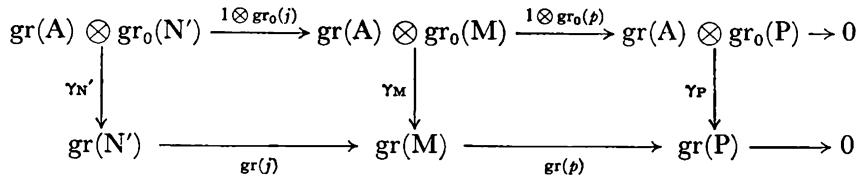
\includegraphics[keepaspectratio]{images/part002_c4775371.jpg}}

the lower row is exact (no. 4, Proposition 2) and so is the upper row by virtue of Proposition 2 of no. 4 and the fact that \(\mathrm{gr}_0(\mathbf{A})\) is a field. Moreover, \(\mathrm{gr}(j)\) is injective (no. 4, Proposition 2) and hence \(\mathrm{gr}_0(j)\) is injective. The first part of the argument applied to \(j\) shows that \(\gamma_{\mathbf{N}'}\) is bijective; as \(\gamma_{\mathbf{M}}\) is also bijective by hypothesis, we conclude that \(\gamma_{\mathbf{P}}\) is bijective (Chapter I, § 1, no. 4, Corollary 2 to Proposition 2).

COROLLARY. Under the hypotheses of Proposition 9, if we assume also that N is Hausdorff with the m-adic filtration, then u is injective.

This follows from the fact that \(\operatorname{gr}(u)\) is injective (Corollary 1 to Theorem 1).

* Remark. Suppose that the hypotheses of Proposition 9 hold and also one of the following conditions:

\begin{enumerate}
\def\labelenumi{(\arabic{enumi})}
\item
  m is nilpotent;
\item
  A is Noetherian and P is ideally Hausdorff (cf.~§ 5, no. 1);
\end{enumerate}

then P is a flat A-module. This follows from the fact that \(\gamma_{P}\) is bijective and § 5, no. 2, Theorem 1 (iv), since A/m is a field. *

